\documentclass[a4paper,12pt]{article}
\usepackage{graphicx}
\usepackage{amsmath}
\usepackage{array}
\usepackage{fancyhdr}
\usepackage{geometry}
\usepackage{titlesec}
\usepackage{circuitikz}
\usepackage{tikz}
\usepackage[T1]{fontenc}
\usepackage[utf8]{inputenc}
\usepackage{karnaugh-map}
\usetikzlibrary{circuits.logic.US, positioning}
\geometry{margin=1in}
\pagestyle{fancy}
\fancyhf{}
\rhead{EE24BTECH11012 - EE24BTECH11019}
\lhead{Experiment - 9}
\cfoot{\thepage}
\titleformat{\section}{\large\bfseries}{\thesection}{1em}{}

\begin{document}

\bibliographystyle{IEEEtran}
\vspace{3cm}

\title{EE1200 - ELECTRIC CIRCUITS LAB \\ \textbf{Experiment-9} }
\author{EE24BTECH11012 - Bhavanisankar G S \\ EE24BTECH11019 - Dwarak A}
% \maketitle
% \newpage
% \bigskip
\begin{center}
    
\includegraphics[width=0.5\textwidth]{IITH.png} \\ % Replace with your logo file
    \vspace{1cm} % Adjust spacing as needed
    \LARGE
    \end{center}
{\let\newpage\relax\maketitle}

\newpage
\tableofcontents
\newpage

\section{Aim}
The objective of this experiment is to build a sequence detector, that detects the sequence of \textbf{11011} by using a \textbf{Moore machine} .

\section{Apparatus Required}
\begin{itemize}
    \item 7474 D flip-flops
    \item 7432 2-input OR gates
    \item 7411 3-input AND gates
    \item LED
    \item Connecting wires
    \item Breadboard
    \item An Ardino UNO
    \item Resistor ( $ 220 \Omega$ )
\end{itemize}

\section{Theory}
A Moore machine is a finite-state machine where the output depends solely on the current state. Key characteristics include:
\begin{itemize}
    \item \textbf{States}: A finite set of states.
    \item \textbf{Input Alphabet}: A set of input symbols.
    \item \textbf{Output Alphabet}: A set of output symbols.
    \item \textbf{State Transition Function}: Maps current state and input to the next state.
    \item \textbf{Output Function}: Maps current state to an output symbol.
\end{itemize}

Formally, a Moore machine is defined as:
\[ M = (Q, \Sigma, \Lambda, \delta, \omega, q_0) \]
where \( Q \) is the set of states, \( \Sigma \) is the input alphabet, \( \Lambda \) is the output alphabet, \( \delta \) is the state transition function, \( \omega \) is the output function, and \( q_0 \) is the initial state.

\subsection*{Advantages:}
\begin{itemize}
    \item Simplicity and stability in output.
    \item Useful in digital circuit design and control systems.
\end{itemize}

\subsection*{Disadvantages:}
\begin{itemize}
    \item May require more states compared to Mealy machines.
    \item Output changes occur one clock cycle after state change.
\end{itemize}

\section{State diagram}
\begin{figure}[!ht]
    \centering
    \resizebox{1\textwidth}{!}{%
    \begin{circuitikz}
        \tikzstyle{every node}=[font=\large]

        \draw  (2.75,17) rectangle (5.5,15);
        \draw  (7.75,17) rectangle (10.75,15);
        \draw  (12.75,17) rectangle (15.75,15);
        \draw  (12.75,13.25) rectangle (15.75,11.25);
        \draw  (7.75,13.25) rectangle (11,11.25);
        \draw  (2.75,13.25) rectangle  node {\LARGE $S_5  | 1$} (5.5,11.25);

        \node [font=\LARGE] at (4,16) {$S_0 | 0$};
        \node [font=\LARGE] at (9.5,16) {$S_1 | 0$};
        \node [font=\LARGE] at (14,16) {$S_2 | 0$};
        \node [font=\LARGE] at (14.25,12.25) {$S_3 | 0$};
        \node [font=\LARGE] at (9.25,12.25) {$S_4 | 0$};

        \draw [->, >=Stealth] (5.5,16) -- (7.75,16);
        \node [font=\large] at (6.5,16.25) {$1$};
        \draw [->, >=Stealth] (10.75,16) -- (12.75,16);
        \node [font=\large] at (11.75,16.25) {$1$};
        \draw [->, >=Stealth] (14,15) -- (14,13.25);
        \draw [->, >=Stealth] (12.75,12.25) -- (11,12.25);
        \draw [->, >=Stealth] (7.75,12.25) -- (5.5,12.25);

        \node [font=\large] at (14.25,14) {$0$};
        \node [font=\large] at (12,12.5) {$1$};
        \node [font=\large] at (6.75,12.5) {$1$};

        \draw (3.5,17) to[short] (3.5,18.75);
        \draw (3.5,18.75) to[short] (4.5,18.75);
        \draw [->, >=Stealth] (4.5,18.75) -- (4.5,17);
        \node [font=\large] at (4,18.5) {$0$};

        \draw [->, >=Stealth] (7.75,15.5) -- (5.5,15.5);
        \node [font=\large] at (6.5,15.25) {$0$};

        \draw (14,17) to[short] (14,18.5);
        \draw (14,18.5) to[short] (14.75,18.5);
        \draw [->, >=Stealth] (14.75,18.5) -- (14.75,17);
        \node [font=\large] at (14.5,18.25) {$1$};

        \draw (13.5,13.25) to[short] (13.5,14);
        \draw (13.5,14) to[short] (4,14);
        \draw [->, >=Stealth] (4,14) -- (4,15);
        \node [font=\large] at (8.75,14.25) {$0$};

        \draw (9,13.25) to[short] (9,13.75);
        \draw (9,13.75) to[short] (3.25,13.75);
        \draw [->, >=Stealth] (3.25,13.75) -- (3.25,15);
        \node [font=\large] at (6.5,13.5) {$0$};

        \draw (2.75,13) to[short] (2,13);
        \draw (2,13) to[short] (2,19.25);
        \draw (2,19.25) to[short] (13.25,19.25);
        \draw (2.75,13) to[short] (2,13);
        \node [font=\large] at (6.5,19) {};

        \draw [->, >=Stealth] (13.25,19.25) -- (13.25,17);
        \node [font=\large] at (8.75,19.5) {$1$};

        \draw (4,11.25) to[short] (4,10.75);
        \draw (4,10.75) to[short] (14,10.75);
        \draw [->, >=Stealth] (14,10.75) -- (14,11.25);
        \node [font=\large] at (9.25,10.5) {$0$};
    \end{circuitikz}
    }
    \caption{State Diagram}
    \label{fig:state_diagram}
\end{figure}

\section{State transition table}
\begin{itemize}
    \item The given sequence, \textbf{11011} has 5 bits. Hence, the required number of states is 6 and the required number of flip-flops to implement this circuit is three.
    \item Let us assign the following binary values to each state - \\
    \begin{table}[ht]
    \centering
    \begin{tabular}{|c|c|}
        \hline
        \textbf{State} & \textbf{Binary value} \\
        \hline
        $S_0$ & $000$ \\
        \hline
        $S_1$ & $001$ \\
        \hline
        $S_2$ & $011$ \\
        \hline
        $S_3$ & $010$ \\
        \hline
        $S_4$ & $110$ \\
        \hline
        $S_5$ & $111$ \\
        \hline
    \end{tabular}
    \caption{State values}
    \label{tab:state_values}
\end{table}
    \item The state-transition table using T flip-flops is given below. \\
    \begin{table}[ht]
    \centering
    \begin{tabular}{|c||c|c|c||c|c|c||c|c|c||c|}
        \hline
        \textbf{Input} & \textbf{$P_{2}$} &  \textbf{$P_1$} & \textbf{$P_0$} & \textbf{$T_2$} & \textbf{$T_1$} & \textbf{$T_0$} & \textbf{$N_2$} & \textbf{$N_1$} & \textbf{$N_0$} & \textbf{Output}\\
        \hline
        0 & 0 & 0 & 0 & 0 & 0 & 0 & 0 & 0 & 0 & 0 \\
        \hline
        1 & 0 & 0 & 0 & 0 & 0 & 1 & 0 & 0 & 1 & 0 \\
        \hline
        0 & 0 & 0 & 1 & 0 & 0 & 1 & 0 & 0 & 0 & 0 \\
        \hline
        1 & 0 & 0 & 1 & 0 & 1 & 0 & 0 & 1 & 1 & 0 \\
        \hline
        0 & 0 & 1 & 1 & 0 & 0 & 1 & 0 & 0 & 1 & 0 \\
        \hline
        1 & 0 & 1 & 1 & 0 & 0 & 0 & 0 & 1 & 1 & 0 \\
        \hline
        0 & 0 & 1 & 0 & 0 & 1 & 0 & 0 & 0 & 0 & 0 \\
        \hline
        1 & 0 & 1 & 0 & 1 & 0 & 0 & 1 & 1 & 0 & 0 \\
        \hline
        0 & 1 & 1 & 0 & 1 & 1 & 0 & 0 & 0 & 0 & 0 \\
        \hline
        1 & 1 & 1 & 0 & 0 & 0 & 1 & 1 & 1 & 1 & 0 \\
        \hline
        0 & 1 & 1 & 1 & 1 & 0 & 1 & 0 & 1 & 0 & 1 \\
        \hline
        1 & 1 & 1 & 1 & 1 & 0 & 0 & 0 & 1 & 1 & 1 \\
        \hline
        0 & 1 & 0 & 0 & X & X & X & X & X & X & X \\
        \hline
        1 & 1 & 0 & 0 & X & X & X & X & X & X & X \\
        \hline
        0 & 1 & 0 & 1 & X & X & X & X & X & X & X \\
        \hline
        0 & 1 & 0 & 1 & X & X & X & X & X & X & X \\
        \hline
        
    \end{tabular}
    \caption{State transition table - T flip-flops}
    \label{tab:state_transiton_table_t}
\end{table} \\
\item The corresponding logic is given below - \\
\begin{table}[ht]
    \centering
    \begin{tabular}{|c|c|}
        \hline
        \textbf{State} & \textbf{Logic} \\
        \hline
        $T_2$ & $Q_2 Q_0 + \overline{I} Q_2 + I \overline{Q_2} Q_1 \overline{Q_0}$ \\
        \hline
        $T_1$ & $\overline{Q_1} Q_0 I + Q_1 \overline{Q_0} \overline{I}$ \\
        \hline
        $T_0$ & $Q_0 \overline{I} + \overline{Q_1} \overline{Q_0} I + I Q_2 \overline{Q_0}$ \\
        \hline
        $O$ & $Q_0 Q_1 Q_2$ \\
        \hline
    \end{tabular}
    \caption{Logic - T flip-flops}
    \label{tab:t_logic}
\end{table}

\item The state transition table using D flip-flops is given below - 
\begin{table}[!ht]
    \centering
    \begin{tabular}{|c||c|c|c||c|c|c||c|c|c||c|}
        \hline
        \textbf{Input} & \textbf{$P_{2}$} &  \textbf{$P_1$} & \textbf{$P_0$} & \textbf{$D_2$} & \textbf{$D_1$} & \textbf{$D_0$} & \textbf{$N_2$} & \textbf{$N_1$} & \textbf{$N_0$} & \textbf{Output}\\
        \hline
        0 & 0 & 0 & 0 & 0 & 0 & 0 & 0 & 0 & 0 & 0 \\
        \hline
        1 & 0 & 0 & 0 & 0 & 0 & 1 & 0 & 0 & 1 & 0 \\
        \hline
        0 & 0 & 0 & 1 & 0 & 0 & 0 & 0 & 0 & 0 & 0 \\
        \hline
        1 & 0 & 0 & 1 & 0 & 1 & 1 & 0 & 1 & 1 & 0 \\
        \hline
        0 & 0 & 1 & 1 & 0 & 0 & 1 & 0 & 0 & 1 & 0 \\
        \hline
        1 & 0 & 1 & 1 & 0 & 1 & 1 & 0 & 1 & 1 & 0 \\
        \hline
        0 & 0 & 1 & 0 & 0 & 0 & 0 & 0 & 0 & 0 & 0 \\
        \hline
        1 & 0 & 1 & 0 & 1 & 1 & 0 & 1 & 1 & 0 & 0 \\
        \hline
        0 & 1 & 1 & 0 & 0 & 0 & 0 & 0 & 0 & 0 & 0 \\
        \hline
        1 & 1 & 1 & 0 & 1 & 1 & 1 & 1 & 1 & 1 & 0 \\
        \hline
        0 & 1 & 1 & 1 & 0 & 1 & 0 & 0 & 1 & 0 & 1 \\
        \hline
        1 & 1 & 1 & 1 & 0 & 1 & 1 & 0 & 1 & 1 & 1 \\
        \hline
        0 & 1 & 0 & 0 & X & X & X & X & X & X & X \\
        \hline
        1 & 1 & 0 & 0 & X & X & X & X & X & X & X \\
        \hline
        0 & 1 & 0 & 1 & X & X & X & X & X & X & X \\
        \hline
        0 & 1 & 0 & 1 & X & X & X & X & X & X & X \\
        \hline
        
    \end{tabular}
    \caption{State transition table - D flip-flops}
    \label{tab:state_transiton_table_d}
\end{table}

\item The corresponding logic is given below - \\
\begin{table}[ht]
    \centering
    \begin{tabular}{|c|c|}
        \hline
        \textbf{State} & \textbf{Logic} \\
        \hline
        $D_2$ & $D \overline{Q_0} (Q_1 + Q_2)$ \\
        \hline
        $D_1$ & $D(Q_0 + Q_1 + Q_2) + Q_1 Q_0$ \\
        \hline
        $D_0$ & $D (Q_0 + Q_2 + \overline{Q_1})$ \\
        \hline
        $O$ & $Q_0 Q_1 Q_2$ \\
        \hline
    \end{tabular}
    \caption{Logic - D flip-flops}
    \label{tab:d_logic}
\end{table}
\item From \ref{tab:t_logic} and \ref{tab:d_logic}, it can be seen that using a D flip-flop minimizes the circuit complexity, and hence we shall adopt that.
\end{itemize}

\section{Circuit diagram}

\begin{figure}[!ht]
\centering
\resizebox{1\textwidth}{!}{%
\begin{circuitikz}
\tikzstyle{every node}=[font=\large]
\draw  (5.5,16.5) rectangle (7.5,13.75);
\draw (17.5,18.25) to[short] (17.5,18);
\draw (18,18.25) to[short] (18,18);
\draw (17.5,18) node[ieeestd and port, anchor=in 2, scale=0.89, rotate=270](port){} (port.out) to[short] (17.75,16.25);
\draw  (10.5,16.5) rectangle (12.25,13.75);
\draw  (14.75,16.5) rectangle (16.5,13.75);
\draw (2.75,12.5) to[short] (13.75,12.5);
\draw (13.75,12.5) to[short] (13.75,14.5);
\draw (13.75,14.5) to[short] (14.75,14.5);
\draw (8.75,12.5) to[short] (8.75,14.5);
\draw (8.75,14.5) to[short] (10.5,14.5);
\draw (4,12.5) to[short] (4,14.5);
\draw (4,14.5) to[short] (5.5,14.5);
\draw (11.5,18.75) to[short] (11.75,18.75);
\draw (11.5,18.25) to[short] (11.75,18.25);
\draw (11.75,18.75) node[ieeestd or port, anchor=in 1, scale=0.89](port){} (port.out) to[short] (13.5,18.5);
\draw (7.5,15.75) to[short] (8,15.75);
\draw (7.5,14.75) to[short] (8,14.75);
\draw (12.25,15.75) to[short] (12.75,15.75);
\draw (12.25,14.75) to[short] (12.75,14.75);
\draw (16.5,16) to[short] (17,16);
\draw (16.5,14.75) to[short] (17,14.75);
\draw (8,15.75) to[short] (8,18.75);
\draw (8,18.75) to[short] (11.5,18.75);
\draw (17,16) to[short] (17,17.5);
\draw (17,17.5) to[short] (10.75,17.5);
\draw (10.75,17.5) to[short] (10.75,18.25);
\draw (10.75,18.25) to[short] (11.75,18.25);
\draw (12.75,14.75) to[short] (13.25,14.75);
\draw (13.25,14.75) to[short] (13.25,17.25);
\draw (13.25,17) to[crossing] (13.25,18);
\draw (13.25,18) to[short] (13.75,18);
\draw (13.75,18.5) to[short] (14,18.5);
\draw (13.75,18) to[short] (14,18);
\draw (14,18.5) node[ieeestd or port, anchor=in 1, scale=0.89](port){} (port.out) to[short] (15.75,18.25);
\draw (13.25,18.5) to[short] (14,18.5);
\draw (4.75,15.75) to[short] (5.5,15.75);
\draw (10,15.75) to[short] (10.5,15.75);
\draw (14.25,16) to[short] (14.75,16);
\draw (2.75,12) to[short] (19.25,12);
\draw (19.25,12) to[short] (19.25,18.25);
\draw (18,18.25) to[short] (19.25,18.25);
\draw (15.75,18.25) to[short] (17.5,18.25);
\draw (17.75,16.25) to[short] (17.25,16.25);
\draw (17.25,16.25) to[crossing] (16.75,16.25);
\draw (16.75,16.25) to[short] (16.75,16.75);
\draw (16.75,16.75) to[short] (14.25,16.75);
\draw (14.25,16.75) to[short] (14.25,16);
\draw (13.25,20) to[short] (13.25,20);
\draw (13.25,19.5) to[short] (13.25,19.5);
\draw (13.25,20) node[ieeestd or port, anchor=in 2, scale=0.89, rotate=180](port){} (port.out) to[short] (11.25,19.75);
\draw (13.25,18.5) to[short] (13.25,19.5);
\draw (12.75,15.75) to[crossing] (13.75,15.75);
\draw (13.75,15.75) to[short] (13.75,17.25);
\draw (13.75,17.25) to[crossing] (13.75,17.75);
\draw (13.75,17.75) to[crossing] (13.75,18.25);
\draw (13.75,18.25) to[crossing] (13.75,18.75);
\draw (13.75,18.75) to[short] (13.75,20);
\draw (13.75,20) to[short] (13.25,20);
\draw (10.5,19.75) to[short] (10.5,19.75);
\draw (10.5,19.25) to[short] (10.5,19.25);
\draw (10.5,19.75) node[ieeestd and port, anchor=in 2, scale=0.89, rotate=180](port){} (port.out) to[short] (8.5,19.5);
\draw (13.75,20) to[short] (13.75,20.75);
\draw (13.75,20.75) to[short] (10.5,20.75);
\draw (10.5,20.75) to[short] (10.5,19.75);
\draw (10.5,18.75) to[short] (10.5,19.25);
\draw (8,20) to[short] (8,20);
\draw (8,19.5) to[short] (8,19.5);
\draw (8,20) node[ieeestd or port, anchor=in 2, scale=0.89, rotate=180](port){} (port.out) to[short] (6,19.75);
\draw (8.5,19.5) to[short] (8,19.5);
\draw (11.25,19.75) to[short] (11.25,20.25);
\draw (11.25,20.25) to[crossing] (9.75,20.25);
\draw (9.75,20.25) to[short] (8,20.25);
\draw (8,20.25) to[short] (8,19.75);
\draw (6,19.75) to[short] (6,17.25);
\draw (6,17.25) to[crossing] (10,17.25);
\draw (10,17.25) to[short] (10,15.75);
\draw (3.25,17.75) to[short] (3.25,17.5);
\draw (3.75,17.75) to[short] (3.75,17.5);
\draw (3.25,17.5) node[ieeestd and port, anchor=in 2, scale=0.89, rotate=270](port){} (port.out) to[short] (3.5,15.75);
\draw (port.left) to[short] (3.5,17.75);
\draw (4.75,20) to[short] (4.75,19.75);
\draw (5.25,20) to[short] (5.25,19.75);
\draw (4.75,19.75) node[ieeestd or port, anchor=in 2, scale=0.89, rotate=270](port){} (port.out) to[short] (5,17.75);
\draw (11,20.75) to[short] (4.75,20.75);
\draw (4.75,20.75) to[short] (4.75,19.75);
\draw (8,18.75) to[short] (6.25,18.75);
\draw (6.25,18.75) to[crossing] (5.75,18.75);
\draw (5.75,18.75) to[short] (5.75,20);
\draw (5.75,20) to[short] (5.25,20);
\draw (5,17.75) to[short] (3.75,17.75);
\draw (2.75,12) to[short] (0.75,12);
\draw (2,12) to[short] (2,18.25);
\draw (2,18.25) to[short] (3.5,18.25);
\draw (3.5,17.75) to[short] (3.5,18.25);
\draw (17,14.75) to[short] (17,12.25);
\draw (17,12.25) to[short] (3.25,12.25);
\draw (3.5,12.25) to[short] (2.25,12.25);
\draw (2.25,12.25) to[short] (2.25,17.75);
\draw (2.25,17.75) to[short] (3.25,17.75);
\draw (3.5,15.75) to[short] (5.25,15.75);
\node [font=\large] at (3.25,12.75) {$Clk$};
\node [font=\large] at (1.5,11.75) {$Input$};
\node [font=\large] at (14.5,15.75) {$D_0$};
\node [font=\large] at (10,15.5) {$D_1$};
\node [font=\large] at (5,15.5) {$D_2$};
\node [font=\large] at (16.75,15.75) {$Q_0$};
\node [font=\large] at (16.75,14.45) {$\overline{Q_0}$};
\node [font=\large] at (12.75,16) {$Q_1$};
\node [font=\large] at (12.5,14.45) {$\overline{Q_1}$};
\node [font=\large] at (7.75,15.5) {$Q_2$};
\node [font=\large] at (7.5,14.45) {$\overline{Q_2}$};
\node [font=\large] at (6.5,15.25) {$FF_2$};
\node [font=\large] at (11.25,15.25) {$FF_1$};
\node [font=\large] at (15.75,15.25) {$FF_0$};
\draw (17,16) to[short] (18.5,16);
\draw (18.5,16) to[short] (18.5,12.25);
\draw (18.5,12.25) to[crossing] (18.5,11.75);
\draw (18.5,11.75) to[short] (20.5,11.75);
\draw (13.75,20.75) to[short] (19.75,20.75);
\draw (19.75,20.75) to[short] (19.75,12);
\draw (19.75,12) to[short] (20.5,12);
\draw (8,15.75) to[short] (9.25,15.75);
\draw (9.25,15.75) to[short] (9.25,14.75);
\draw (9.25,14.75) to[crossing] (9.25,14.25);
\draw (9.25,14.25) to[short] (9.25,12.75);
\draw (9.25,12.75) to[crossing] (9.25,11.5);
\draw (20.5,11.5) to[short] (9.25,11.5);
\draw (20.5,12) to[short] (20.75,12);
\draw (20.5,11.5) to[short] (20.75,11.5);
\draw (20.75,12) node[ieeestd and port, anchor=in 1, scale=0.89](port){} (port.out) to[short] (22.5,11.75);
\draw (port.left) to[short] (20.5,11.75);
\draw (22.25,11.75) to[empty led] (23.25,11.75);
\node [font=\large] at (22.5,12.75) {$Output$};
\end{circuitikz}
}%
\caption{Circuit diagram}
\label{fig:circuit_diag}

\end{figure}

\section{Procedure}

\begin{itemize}
    \item Connect the circuit according to the figure \ref{fig:circuit_diag}.
    \item When the circuit reaches the $S_5$, the LED glows.
    \item The number of times the sequence \textbf{11011} appears can be found out by noting the number of times the LED lights up.
\end{itemize}

\section{Observation}
\begin{itemize}
    \item The simulated diagram is attached herewith - \\
    \begin{figure}[h]
  \centering
  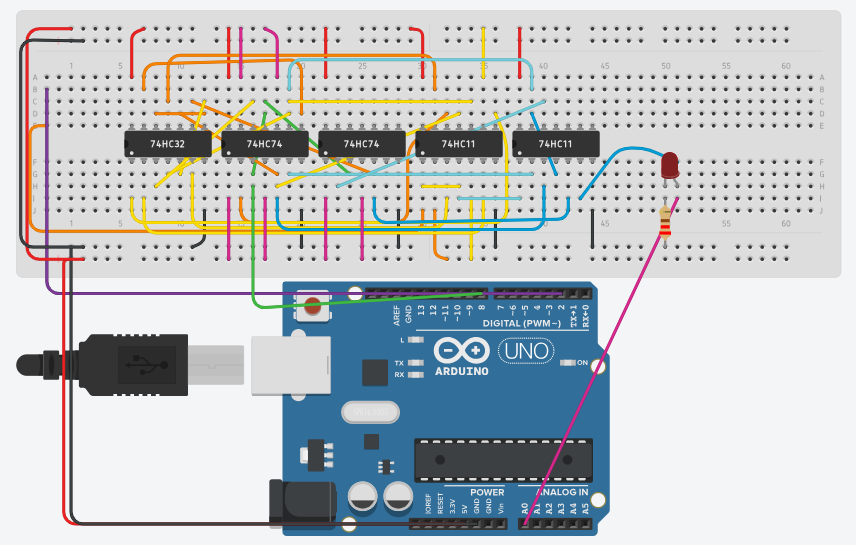
\includegraphics[width=0.6\textwidth]{tinkercad.png}
  \caption{Simulated diagram}
  \label{fig:simulated_diag}
\end{figure}
\item It can be seen that the LED glows 4 times, in an interval of 3 seconds for the bit sequence \textbf{11011011011011011} and 5 seconds for the first time to glow, in one cycle.
\item This can be explained by the nature of the functioning of the Moore machine. When the circuit reaches $S_5$, the LED lights up, which can be seen from the circuit diagram.
\end{itemize}

\section{Result}
Hence, the sequence detector circuit has been constructed using logic gates and D-flip-flops, by a finite state machine ( FSM ) .

\end{document}
